\documentclass{beamer}
%Licença do documento: CC-BY

\usepackage[utf8]{inputenc}
\usepackage{default}
\usepackage{epigraph}
%\usetheme{Ilmenau}
\usecolortheme{crane}
\usepackage{graphicx}
\usepackage{caption}
\usepackage{subcaption}
\usepackage{url}
\usepackage{booktabs}
\usepackage[brazilian]{babel}

\author{RF}
\title{Redes Neurais Artificiais: Raspberry Pi e Python}
\date{\today}


\begin{document}

  \selectlanguage{portuguese}

  \begin{frame}
    \begin{figure}[htpb]
    
\includegraphics[scale=0.8]{salvador-logo.png}
   \end{figure}
  \end{frame}

  \frame{\maketitle}

  \frame{\tableofcontents}


  \begin{frame}
    Licença:\\
    CC-BY\\
    Última versão desse documento:
    
  \end{frame}




  \section{O Raspberry Pi}

    \frame{\sectionpage}
    \begin{frame}{A placa}
      \begin{itemize}
	\item Baixo custo e robusta: projetada para crianças
	\item Movimento Maker e computação física
	\item ARM11, 700MHz, 256 MB RAM, GPU 250 MHz
	\item Suporta Debian GNU/Linux compilado para ARM v6
      \end{itemize}
    \end{frame}

    \begin{frame}{Periféricos}
      \begin{figure}[htpb]
	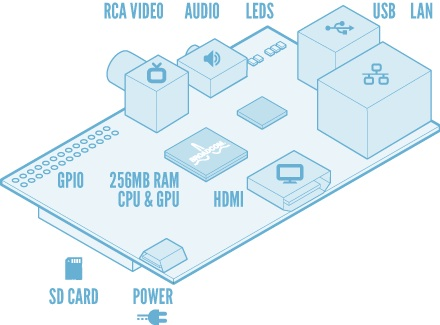
\includegraphics[scale=0.5]{raspberrypi-schematic.jpg}
	\caption{Fonte: \url{raspyfi.com}}
      \end{figure}
    \end{frame}
  \section{Python}
    \frame{\sectionpage}
    
    \begin{frame}{Linguagem Python}
      \begin{itemize}
	\item Linguagem de programação de alto nível, interpretada e orientada a objetos
	\item \texttt{import this}
      \end{itemize}      
    \end{frame}

    \begin{frame}{Tutorial de 2 segundos}
      \texttt{print ``Alô Mundo!!!''}
    \end{frame}
    
  \section{O Campo da Inteligência Computacional}
    \frame{\sectionpage}
      \begin{frame}{O Campo da Inteligência Computacional} 
	Algumas ferramentas que têm amadurecido nos últimos 20 anos tem sido utilizadas com sucesso em problemas até então, intratáveis. A maioria delas é bioinspirada; mimetiza processos que já são conhecidos dos campos da biologia. Podem ser classificadas, basicamente, em 3 áreas:

	\begin{itemize}
	  \item Lógica Fuzzy
	  \item Computação Evolucionária
	  \item Redes Neurais
	\end{itemize}
	Ao contrário da Inteligência Artificial clássica, possui pouca utilização da abordagem simbólica, ênfase em sistemas com computação simples e aprendizado de máquina e não na simulação de agentes inteligentes.
    \end{frame}
  \section{Redes Neurais Artificiais}
    \frame{\sectionpage}
    \subsection{Introdução}
      \begin{frame}{O Cérebro}
	Conforme Haykin, O cérebro pode ser definido como:
	  \begin{quote}
	    Um sistema de processamento de informação altamente complexo, não-linear e paralelo
	  \end{quote}
      \end{frame}
      
      \begin{frame}{O Cérebro}
	Possui as seguintes características:
	\begin{itemize}
	  \item Aprendizagem
	  \item Plasticidade
	  \item Acumula experiência
	  \item É tolerante à falhas
	  \item Processador universal de informação
	\end{itemize} 
      \end{frame}
      
    \subsection{O Neurônio}  
      \begin{frame}{O Neurônio Artificial}
	\begin{figure}[htpb]
	  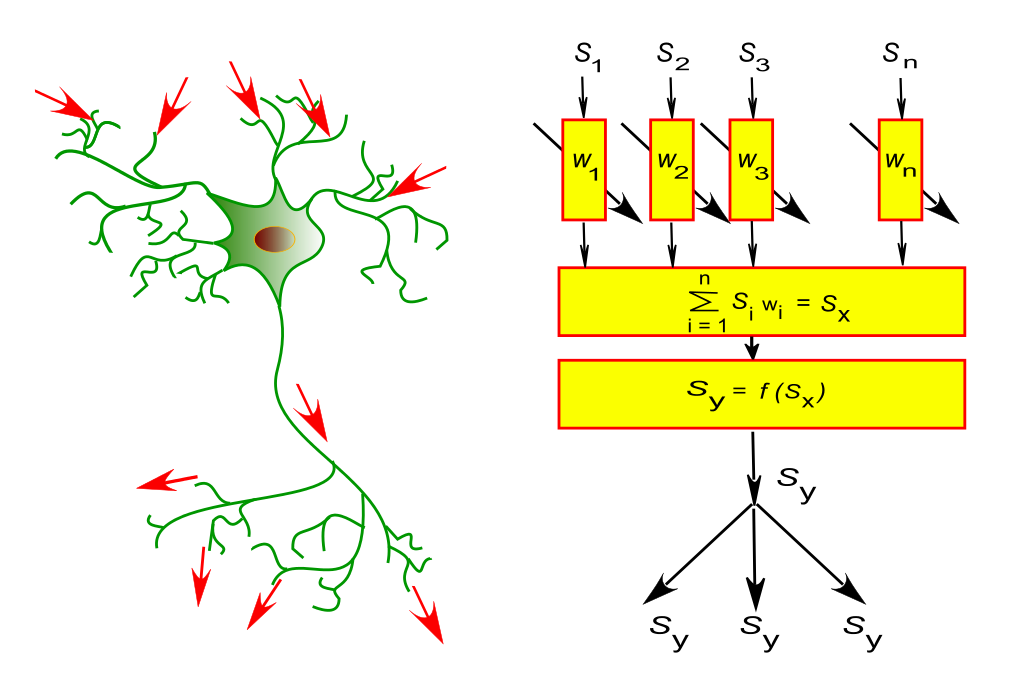
\includegraphics[scale=0.2]{neuronio.png}
	  \caption{Fonte: Wikimedia Commons }
	\end{figure}
      \end{frame}
      
      \begin{frame}{O Neurônio Artificial}
	\begin{figure}[htpb]
	  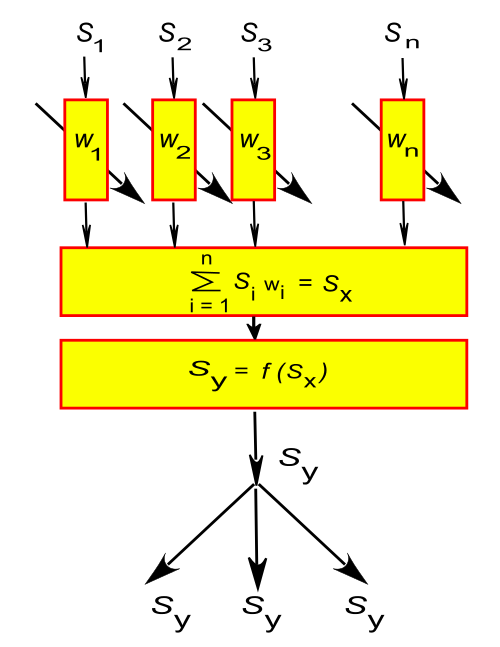
\includegraphics[scale=0.2]{neuronio2.png}
	  \caption{Fonte: Wikimedia Commons }
	\end{figure}
	
	\begin{itemize}
	  \item Entradas
	  \item Pesos
	  \item Somatório
	  \item Campo Local induzido
	  \item Função de Ativação
	\end{itemize}
      \end{frame}
      
      \begin{frame}{Funções de Ativação}
	\begin{figure}[htpb]
	  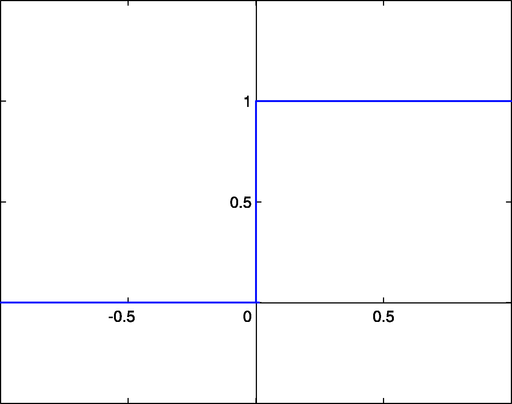
\includegraphics[scale=1.2]{limiar.png}
	  \caption{Função de Limiar. Fonte: Wikimedia Commons }
	\end{figure}
      \end{frame}

      \begin{frame}{Funções de Ativação}
	\begin{figure}[htpb]
	  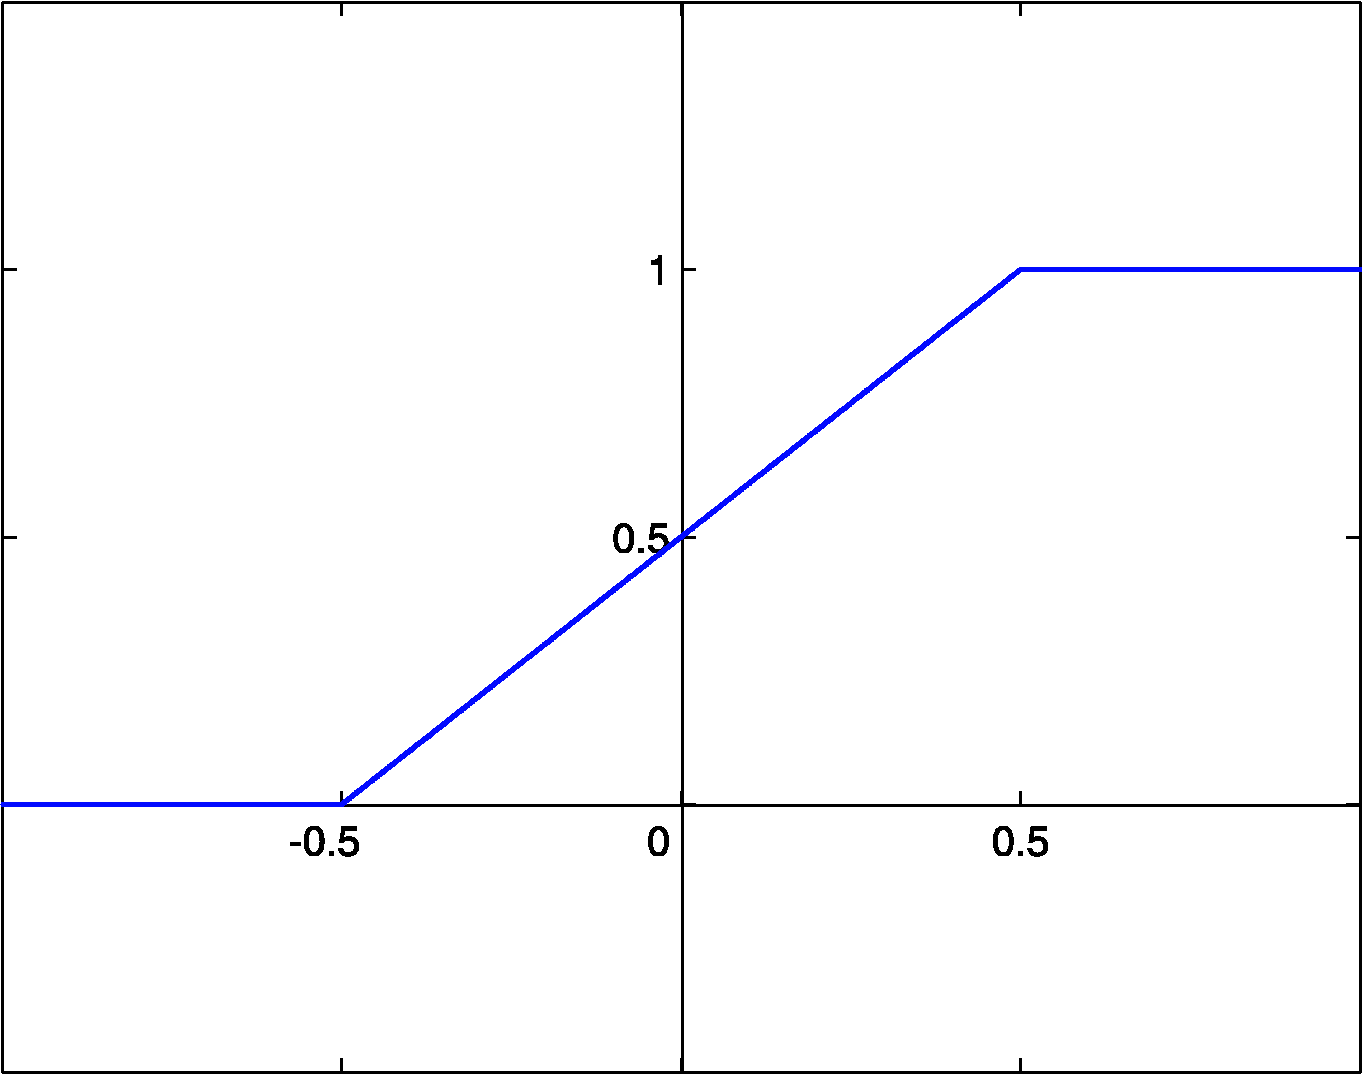
\includegraphics[scale=0.4]{linearpartes.png}
	  \caption{Função Linear por partes. Fonte: Wikimedia Commons }
	\end{figure}
      \end{frame}

      \begin{frame}{Funções de Ativação}
	\begin{figure}[htpb]
	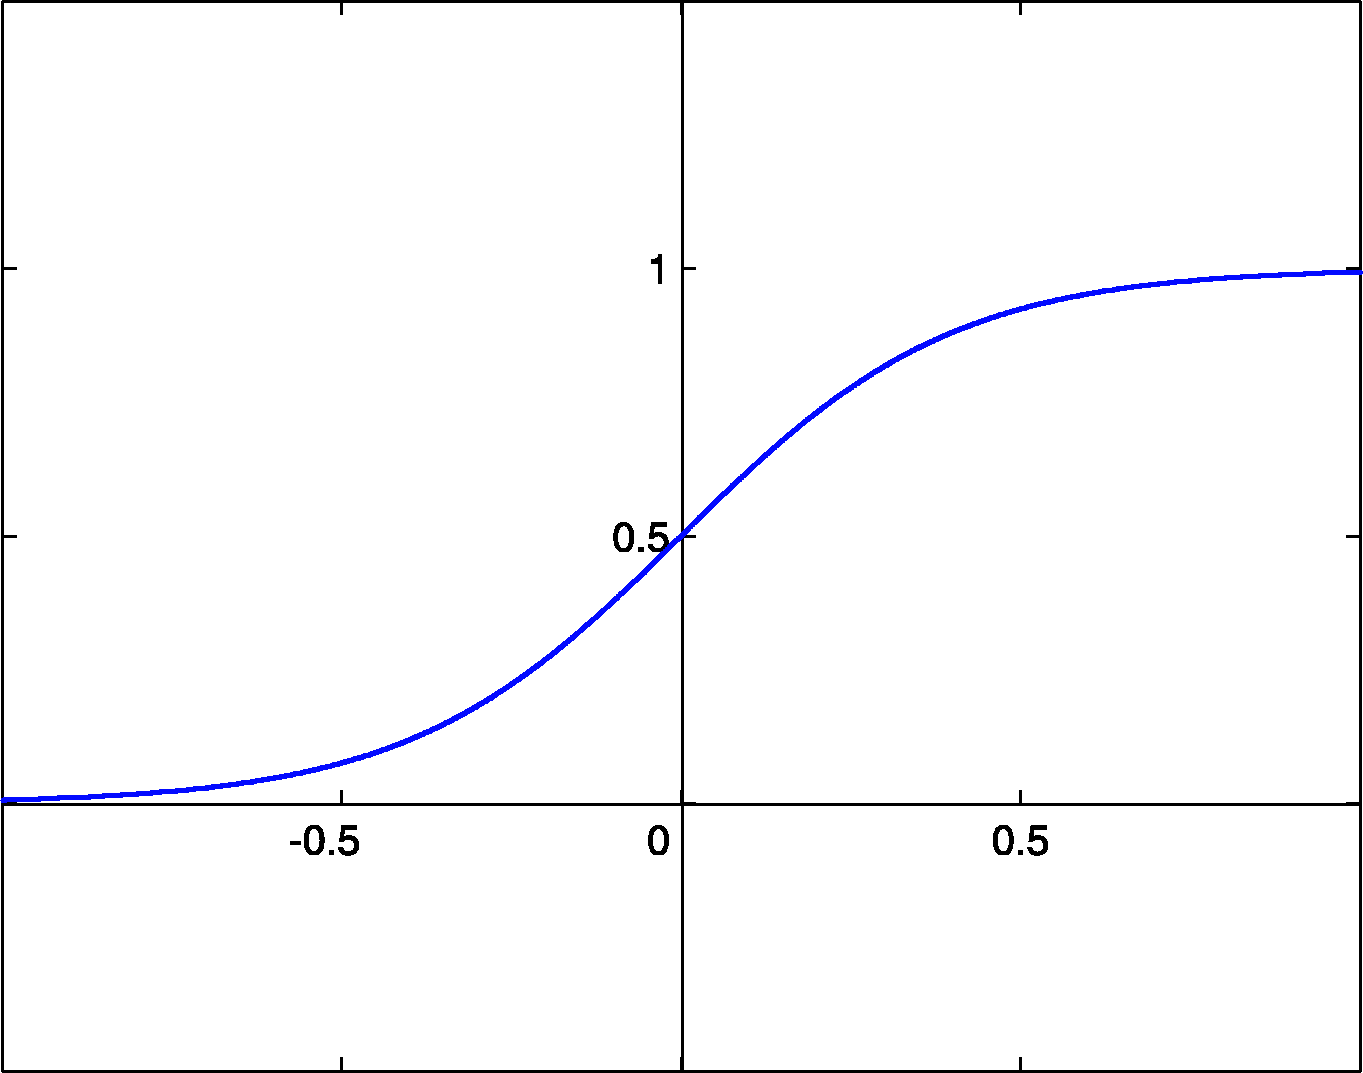
\includegraphics[scale=0.4]{sigmoide.png}
	\caption{Função Sigmóide. Fonte: Wikimedia Commons }
	\end{figure}

	$$\phi (v) = \frac{1}{1 + e^{-av}}$$

      \end{frame}
      
      \begin{frame}{Funções de Ativação}
	\begin{figure}[htpb]
	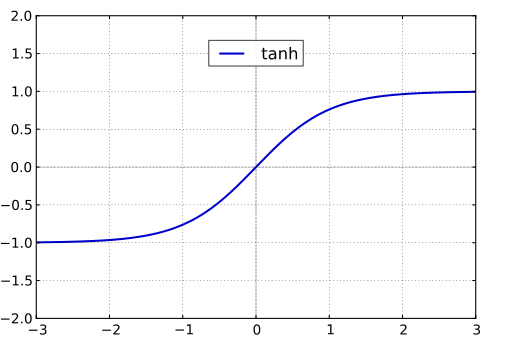
\includegraphics[scale=0.4]{tanh.png}
	\caption{Função tangente sigmóide hiperbólico. Fonte: Wikimedia Commons }
	\end{figure}

	$$\phi (v) = \frac{2}{1 + e^{-2n}} - 1 $$

      \end{frame}
    \subsection{Arquiteturas de Rede}  
      \begin{frame}{A Rede Neural}
	Ainda com Haykin, ele afirma que:
	\begin{quote}
	  Uma Rede Neural é um processador maciçamente paralelamente distribuído constituído de unidades de processamento simples, que tem a propensão natural para armazenar conhecimento experimental e torná-lo disponível para o uso. Ela se assemelha ao cérebro em dois aspectos: O conhecimento é adquirido pela rede a partir de seu ambiente através de um processo de aprendizagem e forças de conexão entre neurônios, conhecidas como pesos sinápticos, são utilizadas para armazenar conhecimento adquirido.
	\end{quote}
      \end{frame}
      
      \begin{frame}{Arquiteturas}
	\begin{figure}[htpb]
	  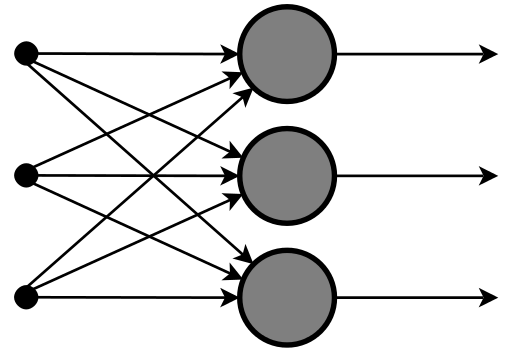
\includegraphics[scale=0.4]{topo1.png}
	  \caption{Redes com uma camada adiante. Fonte: Wikimedia Commons }
	\end{figure}
      \end{frame}

      \begin{frame}{Arquiteturas}
	\begin{figure}[htpb]
	  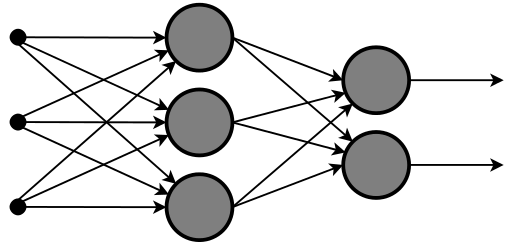
\includegraphics[scale=0.4]{topo3.png}
	  \caption{Redes com múltiplas camadas adiante. Fonte: Wikimedia Commons }
	\end{figure}
      \end{frame}

      \begin{frame}{Arquiteturas}
	\begin{figure}[htpb]
	  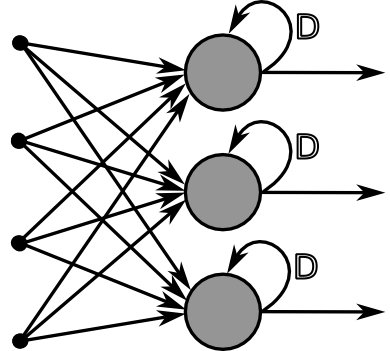
\includegraphics[scale=0.4]{topo2.png}
	  \caption{Redes recorrentes. Fonte: Wikimedia Commons }
	\end{figure}
      \end{frame}
      
    \subsection{Aprendizado de máquina}
  
      \begin{frame}{Definição}
	\begin{quote}
	  Pode-se dizer que um programa de computador aprende de alguma experiência E  com relação a alguma tarefa T e alguma medida de desempenho P, se seu desempenho em T, tal como medido por P , melhora com a experiência E.
	\end{quote}
	Tom Mitchell
    
	Modos: supervisionado e não-supervisionado
      \end{frame}
   
      \begin{frame}{Notação}    
	\begin{figure}[htpb]
	  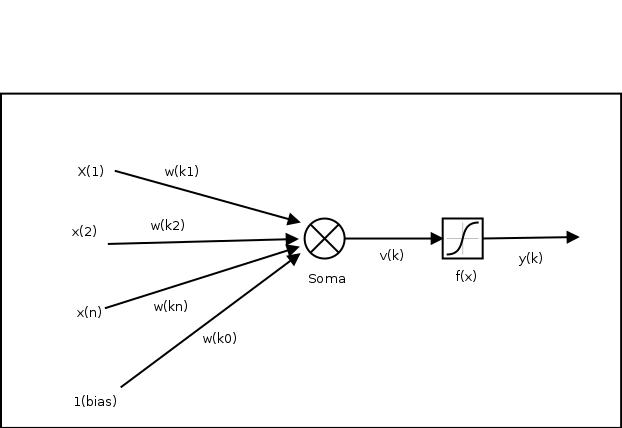
\includegraphics[scale=0.35]{cell.png}
	\end{figure}
    
	\begin{itemize}
	  \item $x_j(n)$: Entrada $j$ do neurônio $k$
	  \item $w_{kj}(n)$: peso da entrada $j$ aplicado ao neurônio $k$ no tempo $n$
	  \item $d_k$: saída desejada pelo professor no tempo $n$.
	  \item $b_k$: \textit{bias} do neurônio $k$.
	\end{itemize}
      \end{frame}
      
      \begin{frame}{Aprendizagem por Correção de erro}
	A comparação entre a saída $y_k$ e a saída apresentada pelo professor $d_k$ gera o erro:
	$$e_k = d_k - y_k$$
  
	Define-se uma função de custo:
  
	$$E(n)= \frac{1}{2} {e_k}^2(n)$$
  
	E realiza-se a minimização de $E(n)$ alterando os pesos da seguinte forma:
  
	$$w_{kj}(n+1) = w_{kj}(n) + \Delta w_{kj}(n+1) $$
	$$\Delta w_{kj}(n) = \eta {e_k}(n)  x_j(n)$$
    
      \end{frame}
  \section{Biblioteca PyBrain}
    \frame{\sectionpage}
    
    \begin{frame}{PyBrain}
      \url{http://pybrain.org/docs/}
      \begin{figure}[htpb]
	
\includegraphics[scale=0.5]{logo_pybrain.png}
      \end{figure}
    \end{frame}
    
    \begin{frame}{Módulos}
      \begin{figure}[htpb]
	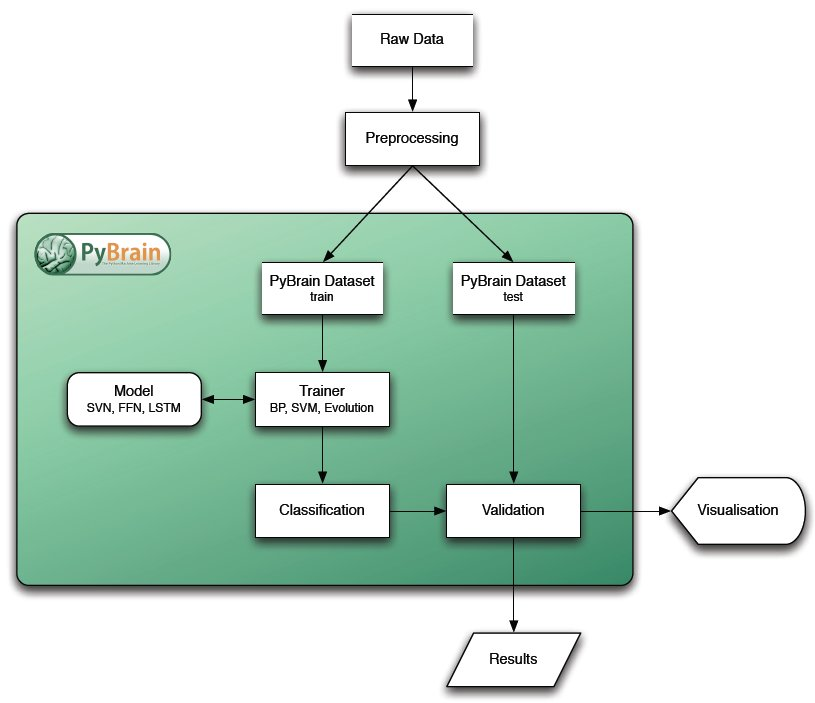
\includegraphics[scale=0.28]{dataprocessing_flowchart.jpg}
	\caption{\url{http://pybrain.org/docs/tutorial/intro.html}}
      \end{figure}
    \end{frame}
    
  \section{Desenvolvimento de Sistemas Utilizando RNA's}
    \frame{\sectionpage}
      \begin{frame}{Etapas de desenvolvimento}
      \begin{itemize}
	\item Definição do problema
	\item Coleta de dados
	\item Pré-tratamento. Normalmente, $\mu = 0$ e $\sigma = 1$.
	\item Configuração da rede
	\item Treinamento
	\item Teste
	\item Integração
      \end{itemize}
    \end{frame}
      
    \begin{frame}{Coleta de dados}
      \begin{figure}[htpb]
	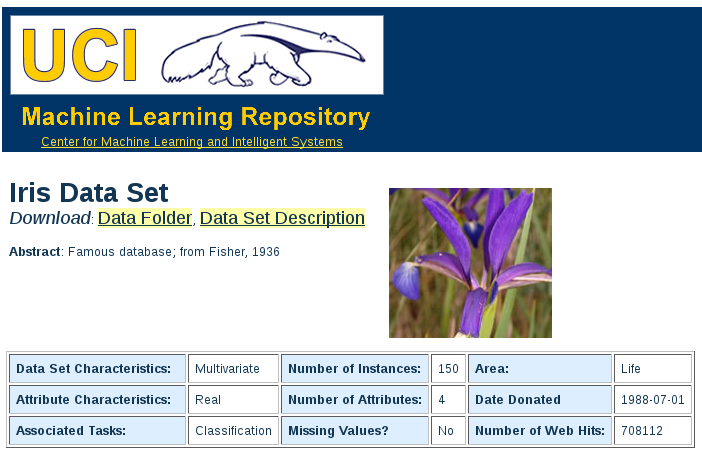
\includegraphics[scale=0.4]{machine.png}
	\caption{Repositório de dados}
      \end{figure}
      \url{http://archive.ics.uci.edu/ml/}
    \end{frame}
    
    \begin{frame}{Separação dos conjuntos de dados}
      \begin{figure}[htpb]
	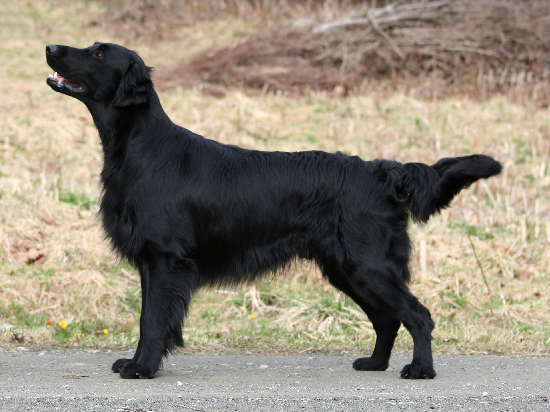
\includegraphics[width=3in]{dog1.jpg}
	\caption{Fonte: Wikimedia Commons}
      \end{figure}
    \end{frame}

    \begin{frame}{Separação dos conjuntos de dados}
      \begin{figure}[htpb]
	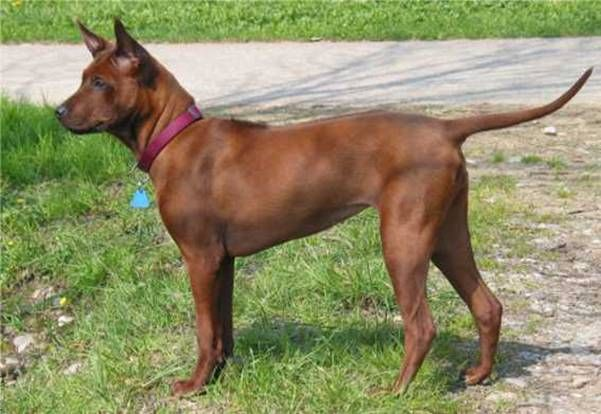
\includegraphics[width=3in]{dog2.jpg}
	\caption{Fonte: Wikimedia Commons}
      \end{figure}
    \end{frame}
    
    \begin{frame}{Separação dos conjuntos de dados}
      \begin{figure}[htpb]
	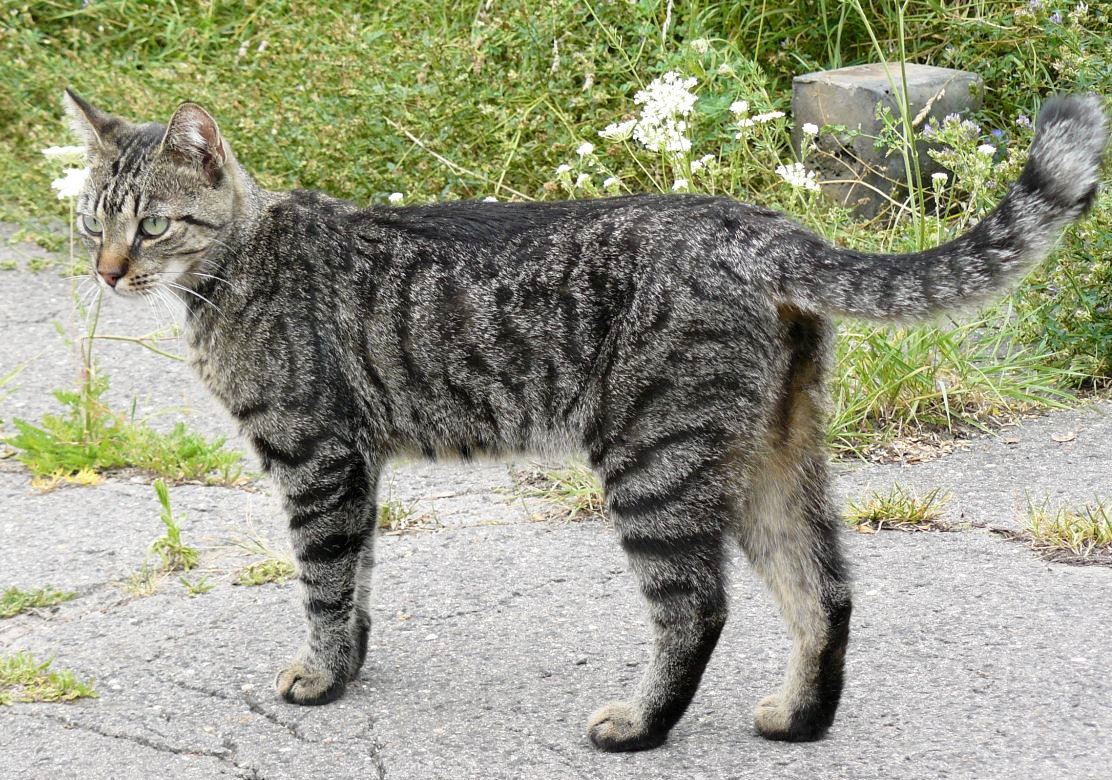
\includegraphics[width=3in]{dog3.jpg}
	\caption{Fonte: Wikimedia Commons}
      \end{figure}
    \end{frame}
    
    \begin{frame}{Separação dos conjuntos de dados}
      \begin{figure}[htpb]
	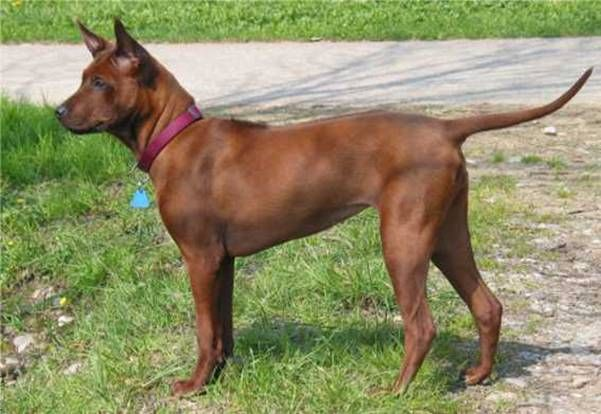
\includegraphics[width=3in]{dog2.jpg}
	\caption{Fonte: Wikimedia Commons}
      \end{figure}
    \end{frame}
    
    \begin{frame}{Separação dos conjuntos de dados}
      \begin{figure}[htpb]
	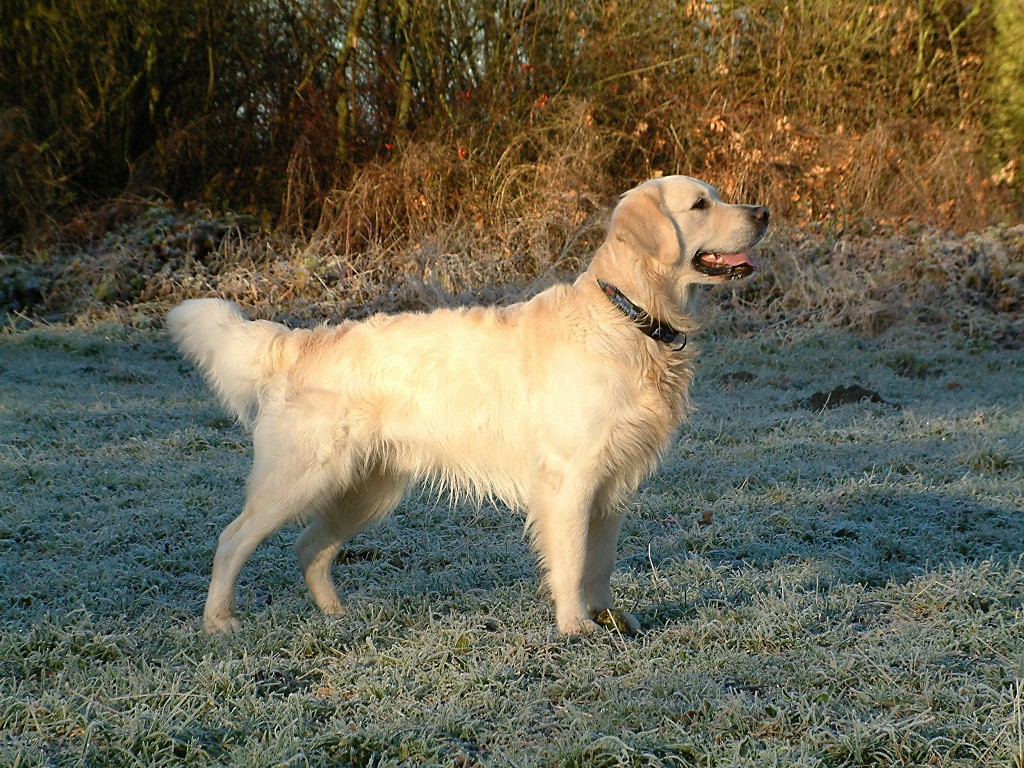
\includegraphics[width=3in]{dog4.jpg}
	\caption{Fonte: Wikimedia Commons}
      \end{figure}
    \end{frame}
    
    \begin{frame}{Separação dos conjuntos de dados}
      Não se pode validar ou testar a rede com os dados utilizados para aprendizado. Separamos os dados em 3 conjuntos:
      \begin{itemize}
	\item Treinamento - Utilizado para realizar o aprendizado através do algoritmo escolhido
	\item Validação - Utilizado para verificar a eficácia da rede e capacidade de generalização.
	\item Teste  - Utilizado para quaisquer testes que o desenvolvedor deseje.
      \end{itemize}
    \end{frame}

  \section{Hands On}
    \frame{\sectionpage}
    
  \nocite{haykin, michell, isaias, faceli, ng, braga}
 
  \section{Bibliografia Recomendada}
  \begin{frame}[allowframebreaks]
    \frametitle{Referências}
    \bibliographystyle{amsalpha}
    \bibliography{apr.bib}
  \end{frame}
\end{document}
